\chapter{実験}
複数タスクにかかる所要時間に対し被験者の予測とADLoggerの予測の差異を比較した上で,
ADLogger導入によって,行動・意識の変容が生じるかどうか検証を実施した.
本章ではまず実験の目的と手法を説明し,得られた実験結果のデータの概要を示す.

\section{実験目的}
本研究では,複数タスクにかかる所要時間の予測に関して被験者の予測とADLoggerの予測の差異を比較する事,
ADLogger導入によって,時間管理に対する苦手意識・行動への変化が起こる事を目的としている.

\section{実験手法}
今回の評価実験では,被験者に時間の長さを教示し,その長さを産生させる時間産生法\cite{Oguro1961}\cite{Tayama2018}を慶應義塾大学の学生男女20名に対し平日と休日(またはそれに準ずる日)にそれぞれ3回(合計6回)に渡って実施した.
始めに,被験者は事前に各自保持しているiPhoneにADLoggerをインストールして貰う.

実験は平日と休日(またはそれに準ずる日)は異なる動き・見積もりを行う可能性を鑑み,3回分の平日と休日をそれぞれ1回ずつ以上(計6回以上)実施した.
被験日はまず行動前に朝実施する日常生活動に関して行動名,行動毎の必要時間予測,タスクを連続で行った時の総合必要時間予測を申告してもらう.
尚,6回の計測を通じて予測を適宜修正できるものとする.
その後,web会議ツールであるzoom\cite{zoom}およびADLoggerを用いながら実際に行動して貰い実測値を計測する.
zoomにおいては全ての行動の開始時/終了時に連絡を行い,実験者が総合時間を計測する.
更に被験者はADLoggerを用いて行動毎の時間を計測する.
一定期間後(原則4回目)以降の計測はADLoggerのADLoggerおよびタイマーのカウントアップ表示を閲覧できる状態にしながら計測して貰う.
最終日にはアプリケーションによる定性的効果やアプリケーションの改善点を知る為にインタビューを行う.インタビューにて質問する項目は付録Aにて記載した.

\section{実験結果}
被験者20名中,被験に協力頂いたのは19名だった.
内,被験期間内に実験を終わらせられた(被験回数6回以上,ADLoggerの効果比較済)のは16名だった.
具体的なユーザ別日程数の内訳は図~\ref{tb:day}に記載した.

\begin{table}[ht]
\begin{center}
 \caption{ユーザ 別被験日数一覧}
\begin{tabular}{|c|c|c|} \hline
Username& Before& After \\\hline
A& 2&1 \\\hline
B& 4&3 \\\hline
C& 2&1 \\\hline
D& 2&1 \\\hline
E& 4&0 \\\hline
F& 5&4 \\\hline
G& 2&1 \\\hline
H& 2&1 \\\hline
I& 2&1 \\\hline
J& 2&1 \\\hline
K& 3&2 \\\hline
L& 4&2 \\\hline
M& 4&2 \\\hline
N& 3&4 \\\hline
O& 3&2 \\\hline
P& 4&4 \\\hline
Q& 2&3 \\\hline
R& 2&0 \\\hline
S& 2&0 \\\hline
\end{tabular}
  \label{tb:day}
\end{center}
\end{table}

また,被験者が行う行動・行動時間は被験者に合わせている為,行動時間には個人差がある.
図~\ref{fig:day}上部はタスク別,下部は合計時間の分布を箱髭図で描いたものであり,被験者の行動時間は個人差が大きい.
タスクは30秒程度のものから30分程度のものまで存在し,合計時間は10分弱から1時間程度である.

\begin{figure}[ht]
	\begin{center}
	\fbox{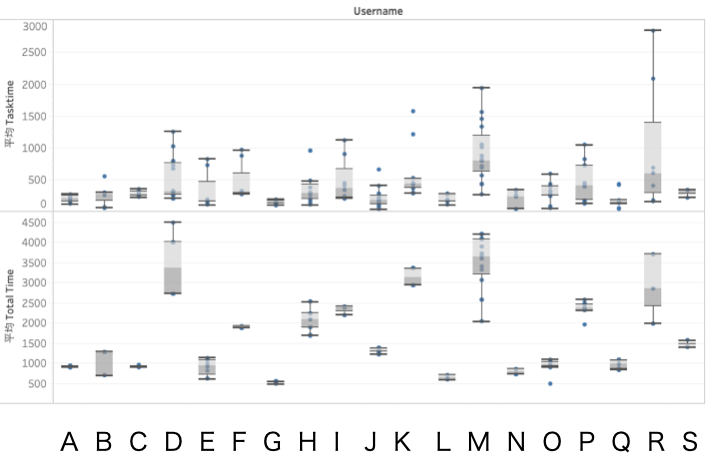
\includegraphics[width=15cm]{images/7/2.png}}
		\caption{ユーザ別行動時間分布}
		\label{fig:day}
	\end{center}
\end{figure}

さらに,ADLogger導入前のタスク別予測と実測の平均時間の比較を図~\ref{fig:compare}に,総合時間の比較を図~\ref{fig:compare2}に記す.
図~\ref{fig:compare},~\ref{fig:compare2}は横軸を実測の平均時間,縦軸を予測の平均時間にしたものである.
見積もりの予測と実態に関して切片が0の一次関数で表すと,図~\ref{fig:compare}はy=0.96x,図~\ref{fig:compare2}はy=0.99xになった.
この事から被験者を全体で見ると予定の予測をぴったりかやや実測より短めに見積もる傾向がある事が分かる.
また,図~\ref{fig:compare3}は図~\ref{fig:compare}の結果を,図~\ref{fig:compare4}は図~\ref{fig:compare2}の結果をユーザ別に傾向線を引いたものである.
被験者は図~\ref{fig:compare3}は係数1.93から0.69の間で,図~\ref{fig:compare3}は係数1.55から0.73の間で見積もっていた.

\begin{figure}[ht]
	\begin{center}
	\fbox{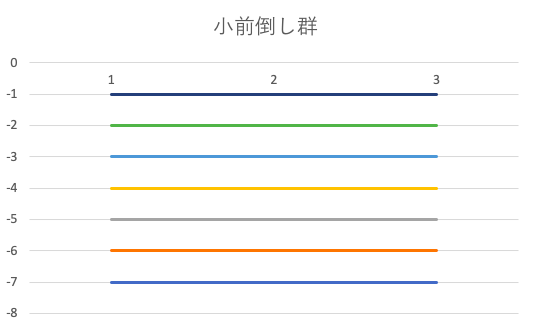
\includegraphics[width=15cm]{images/7/3.png}}
		\caption{予測と実測の平均時間比較}
		\label{fig:compare}
	\end{center}
\end{figure}

\begin{figure}[ht]
	\begin{center}
	\fbox{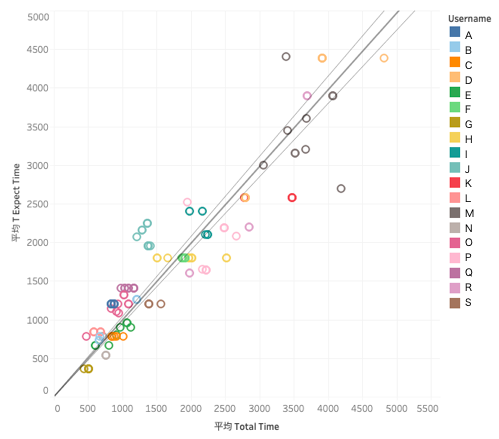
\includegraphics[width=15cm]{images/7/4.png}}
		\caption{予測と実測の平均時間比較(総合時間)}
		\label{fig:compare2}
	\end{center}
\end{figure}

\begin{figure}[ht]
	\begin{center}
	\fbox{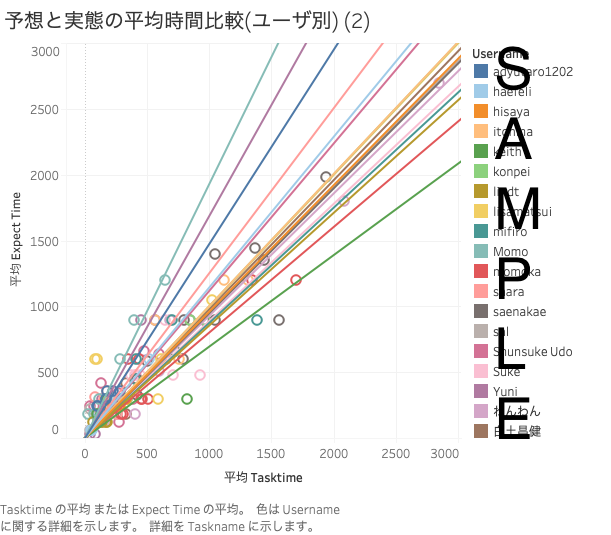
\includegraphics[width=15cm]{images/7/5.png}}
		\caption{予測と実測の平均時間比較(ユーザ別)}
		\label{fig:compare3}
	\end{center}
\end{figure}

\begin{figure}[ht]
	\begin{center}
	\fbox{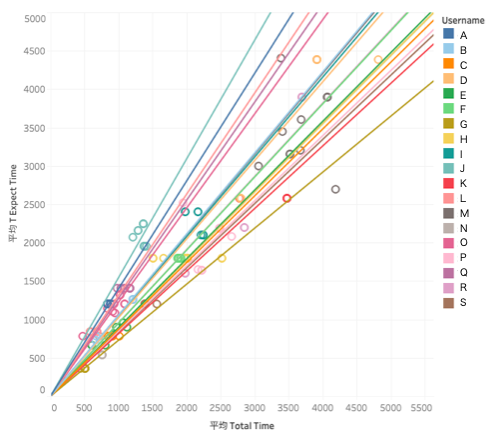
\includegraphics[width=15cm]{images/7/6.png}}
		\caption{予測と実測の平均時間比較(ユーザ別総合時間)}
		\label{fig:compare4}
	\end{center}
\end{figure}

最後にインタビューは途中で実験が終了した3人を除く16名に答えてもらった.
結果の概要は表~\ref{tb:interview}の通りとなった.

\begin{table}[ht]
\begin{center}
 \caption{インタビュー概要}
\begin{tabular}{|c|c|c|c|c|c|c|c|c|c|c|c|c|c|} \hline
匿名 & 変更 & 問1 & 問2 & 問3 & 問4 & 問5 & 問6 & 問7 & 問8 & 問9 & 問10 & 問11 & 問13\\\hline
J & × & 長 & × & × & △ & ○ & × & ○ & ○ & × & やや急ぎ & ○ & ○\\\hline
Q & ○ & 長 & × & × & × & ○ & × & ○ & ○ & × & やや急ぎ & ○ & ○ \\\hline
A & ○ & 定 & × & × & × & ○ & × & × & ○ & × & ゆっくり & ○ & △\\\hline
L & × & 短 & × & × & ○ & ○ & ○ & × & ○ & ○ & ややゆっくり & ○ & ○\\\hline
B & × & 長 & × & × & △ & ○ & ○ & × & ○ & ○ & ゆっくり & ○ & △ \\\hline
O & × & 定 & × & ○ & × & × & ○ & ○ & × & ○ & ゆっくり & ○ & △ \\\hline
D & × & 定 & × & × & ○ & ○ & ○ & × & ○ & × & ゆっくり & ○ & ○ \\\hline
F & × & 長 & × & × & ○ & ○ & ○ & × & ○ & × & ややゆっくり & ○ & ○ \\\hline
H & × & 定 & × & ○ & ○ & ○ & ○ & ○ & × & × & ゆっくり & × & × \\\hline
S & × & 定 &  &  &  &  &  &  &  &  &  &  & \\\hline
C & × & 定 & × & × & × & ○ & × & × & ○ & × & ゆっくり & ○ & △ \\\hline
N & ○ & 定 & × & × & ○ & × & ○ & ○ & × & × & ゆっくり & ○ & × \\\hline
M & ○ & 長 & × & × & △ & ○ & ○ & × & ○ & ○ & ゆっくり & ○ & ×\\\hline
R & × &  &  &  &  &  &  &  &  &  &  &  & \\\hline
P & ○ & 定 & × & × & × & × & ○ & ○ & ○ & × & ゆっくり & ○ & △\\\hline
I & ○ & 長 & × & × & ○ & ○ & × & × & ○ & × & ややゆっくり & ○ & △ \\\hline
G & × & 定 & × & × & ○ & ○ & × & × & ○ & × & ゆっくり & ○ & ○\\\hline
K & × & 短 & × & × & ○ & ○ & ○ & × & ○ & ○ & やや急ぎ & ○ & ○ \\\hline
E & × & 定 &  &  &  &  &  &  &  &  &  &  &\\\hline
\end{tabular}
  \label{tb:interview}
\end{center}
\end{table}

\chapter{評価}
\section{実験評価手法}
本研究はTableau\cite{tableau}を用いて下記の通り評価を行う.
まずアプリケーションの介入によって見積もりと実測の差がどれだけ変化したか全体の比較を行う.
その後,図~\ref{fig:compare}の見積もりの係数が高い順位で並べそれぞれ変化をみた.
上位6人をグループ\UTF{2460},中位上位6人をグループ\UTF{2461},下位7人をグループ\UTF{2462}とした上で
それぞれの見積もり傾向とアプリケーションによる効果の有無を調査する.

\section{評価結果}
本節では,本システムのADLogger機能導入後時間管理に対し与える影響について,本評価実験で得られた評価結果を示す.
\subsection{アプリケーションによる効果}
アプリケーションのADLogger機能を導入する前と後によって係数がどう変化したかを表~\ref{tb:test1}で表した.
表~\ref{tb:test1}は左からタスクごとの時間予測前後、総合時間の前後を表している
表~\ref{tb:test1}の値の数値の欄からわかる様にタスク時間,総合時間ともに係数は減少した.
また被験者の内訳に関しては表~\ref{tb:test2},表~\ref{tb:test3}に表した.
表~\ref{tb:test1},表~\ref{tb:test2},表~\ref{tb:test3}のp値は0.0001より小さい.

また,表~\ref{tb:test4},表~\ref{tb:test5},表~\ref{tb:test6}は図~\ref{fig:compare3}で可視化されたADLogger導入前のタスクごとの時間において
係数が高い被験者順に並べ,それぞれの値の詳細を記した表であり,上からタスク時間,総合時間を導入前,導入後で並べてある.
表~\ref{tb:test4},表~\ref{tb:test5},表~\ref{tb:test6}の値の欄から分かる様に係数が高くなった被験者がいるものの,係数が下振れした被験者の方が多かった.
また,ユーザ別のその他詳細は表~\ref{tb:test7}に表した.

更に係数比較だけではなく,箱髭図から分布を図~\ref{fig:10}にて表した.
表~\ref{fig:10}はタスク時間の秒数での分布,\%での分布,総合時間の秒数での分布,\%での分布を表しており,それぞれADLogger導入前後の比較が出来る.
全ての分布はADLogger導入後の方が分布が狭まり,総合時間に関しては中央値の値がやや高くなった事が分かる.
尚,ADLogger導入後に見積もりの時間を変更したのは3人である.

また,被験者別の使用前後の比較分布を可視化したところタスク時間の秒数分布は図~\ref{fig:11},タスク時間の\%分布は図\ref{fig:12},
総合時間の秒数分布は図~\ref{fig:13},総合時間の\%分布は図~\ref{fig:14}の様になった.
それぞれ効果の度合い,どこの観点から効果が出ているかは個人差が出るが,多くの被験者に誤差の縮小が認められた.


\begin{table}[ht]
\centering
 \caption{ADLogger機能導入前後の係数の比較(総合)2}
\begin{tabular}{|c|c|c|c|c|c|} \hline
行 & p値 & DF  & 値 & 標準誤差 & t 値 \\\hline
Tasktime Before &\verb|<| 0.0001 & 159  & 0.955782 & 0.0231274 & 41.3269\\\hline
Total Time Before  &\verb|<| 0.0001 & 159  & 0.993547 & 0.0223607 & 44.4326 \\\hline
Tasktime After  &\verb|<|0.0001 & 123 \ & 0.955497 & 0.0314031 & 30.4268 \\\hline
Total Time After &\verb|<|0.0001 & 123 &  0.954642 & 0.0132156 & 72.2362\\\hline
\end{tabular}
  \label{tb:test1}
\end{table}

\begin{table}[ht]
\begin{center}
 \caption{ADLogger機能導入前後の係数の比較(総合)1}
\begin{tabular}{|c|c|c|c|c|} \hline
名称 & Tasktime Before & Total Time Before& Tasktime After & Total Time After \\\hline
モデル化された観測の数: & 160 & 160 & 124 & 124 \\\hline
モデルの自由度: & 1 & 1 & 1 & 1 \\\hline
残差の自由度 (DF): & 159 & 159 & 123 & 123 \\\hline
SSE (合計二乗誤差): & 4.78E+06 & 5.90E+07 & 3.83E+06 & 1.23E+07 \\\hline
MSE (平均二乗誤差): & 30037.2 & 370934 & 31105.7 & 100359 \\\hline
R-2 乗: & 0.914833 & 0.925466 & 0.882722 & 0.976971 \\\hline
標準誤差: & 173.312 & 609.043 & 176.368 & 316.794 \\\hline
p 値 (基準値): & \verb|<|0.0001 & \verb|<|0.0001 & \verb|<|0.0001 & \verb|<|0.0001\\\hline
\end{tabular}
  \label{tb:test2}
\end{center}
\end{table}

\begin{table}[ht]
\begin{center}
 \caption{ADLogger導入前後の係数の比較(ユーザ別1)}
\begin{tabular}{|c|c|c|c|c|} \hline
名称 & Tasktime Before & Total Time Before & Tasktime After & Total Time After \\\hline
モデル化された観測の数: & 160 & 160 & 124 & 124 \\\hline
フィルターされた観測の数: & 0 & 0 & 0 & 0 \\\hline
モデルの自由度: & 19 & 19 & 16 & 16 \\\hline
残差の自由度 (DF): & 141 & 141 & 108 & 108 \\\hline
SSE (合計二乗誤差): & 3.21E+06 & 4.22E+07 & 2.98E+06 & 6.62E+06 \\\hline
MSE (平均二乗誤差): & 22773.3 & 299472 & 27610.5 & 61261.8 \\\hline
R-2 乗: & 0.942738 & 0.946638 & 0.908595 & 0.987657 \\\hline
標準誤差: & 150.908 & 547.241 & 166.164 & 247.511 \\\hline
p 値 (基準値): &\verb|<| 0.0001 & \verb|<|0.0001 & \verb|<| 0.0001 & \verb|<| 0.0001 \\\hline
\end{tabular}
  \label{tb:test3}
\end{center}
\end{table}


\begin{table}[ht]
\begin{center}
 \caption{ADLogger導入前後の係数の比較(ユーザ別3)1位から8位}
\begin{tabular}{|c|c|c|c|c|c|c|c|c|} \hline
No. & Username & p 値 & DF & 条件 & 値 & 標準誤差 & t 値 & p 値 \\\hline
1 & J & \verb|<| 0.0001 & 10 & 平均 Tasktime & 1.92944 & 0.0937246 & 20.5863 & \verb|<|0.0001 \\\hline
 &  & \verb|<| 0.0001 & 10 & 平均 Total Time & 1.54632 & 0.0403262 & 38.3452 & \verb|<|0.0001 \\\hline
 &  & \verb|<| 0.0001 & 8 & 平均 Tasktime & 1.06984 & 0.110302 & 9.69922 & \verb|<| 0.0001 \\\hline
 &  & \verb|<| 0.0001 & 8 & 平均 Total Time & 1.09579 & 0.0427638 & 25.6242 & \verb|<| 0.0001\\\hline
2 & Q & \verb|<| 0.0001 & 8 & 平均 Tasktime & 1.6865 & 0.105067 & 16.0516 &\verb|<| 0.0001\\\hline
 &  & N/A & 8 & 平均 Total Time & 1.27716 & * &  &  \\\hline
 &  & \verb|<| 0.0001 & 7 & 平均 Tasktime & 1.65899 & 0.0583316 & 28.4406 & \verb|<| 0.0001 \\\hline
 &  & N/A & 7 & 平均 Total Time & 1.27876 & * &  &  \\\hline
3 & A & \verb|<|0.0001 & 7 & 平均 Tasktime & 1.47383 & 0.147837 & 9.96928 & \verb|<| 0.0001 \\\hline
 &  & N/A & 7 & 平均 Total Time & 1.40227 & * &  &  \\\hline
 &  & \verb|<| 0.0001 & 7 & 平均 Tasktime & 1.39344 & 0.0977549 & 14.2544 &\verb|<| 0.0001\\\hline
 &  & N/A & 7 & 平均 Total Time & 1.18316 & * &  &  \\\hline
4 & L & 0.0080992 & 5 & 平均 Tasktime & 1.25206 & 0.294669 & 4.24905 & 0.0080992 \\\hline
 &  & N/A & 5 & 平均 Total Time & 1.31654 & * &  &  \\\hline
 &  & 0.0251471 & 5 & 平均 Tasktime & 1.23513 & 0.391091 & 3.15816 & 0.0251471\\\hline
 &  & N/A & 5 & 平均 Total Time & 1.28689 & * &  & \\\hline
5 & B & \verb|<| 0.0001 & 6 & 平均 Tasktime & 1.14357 & 0.02087 & 54.7949 &\verb|<|0.0001 \\\hline
 &  &\verb|<| 0.0001 & 6 & 平均 Total Time & 1.05631 & 0.0145376 & 72.6607 &\verb|<|0.0001 \\\hline
 &  &\verb|<|0.0001 & 6 & 平均 Tasktime & 1.03551 & 0.0634924 & 16.3092 & \verb|<| 0.0001 \\\hline
 &  & \verb|<| 0.0001 & 6 & 平均 Total Time & 0.942548 & 0.0057161 & 164.893 & \verb|<|0.0001 \\\hline
6 & O & 0.000142 & 8 & 平均 Tasktime & 1.11809 & 0.165136 & 6.77069 & 0.000142 \\\hline
 &  & \verb|<| 0.0001 & 8 & 平均 Total Time & 1.22626 & 0.0407566 & 30.0873 & \verb|<|0.0001 \\\hline
 &  & 0.0062528 & 3 & 平均 Tasktime & 1.43583 & 0.208268 & 6.89416 & 0.0062528 \\\hline
 &  & N/A & 3 & 平均 Total Time & 1.28459 & * &  & \\\hline
7 & D & \verb|<|0.0001 & 11 & 平均 Tasktime & 1.00217 & 0.056799 & 17.6442 & \verb|<|0.0001\\\hline
 &  & \verb|<| 0.0001 & 11 & 平均 Total Time & 1.02381 & 0.0305331 & 33.5312 & \verb|<|0.0001\\\hline
 &  &\verb|<|0.0001 & 11 & 平均 Tasktime & 0.992669 & 0.0781869 & 12.6961 & \verb|<|0.0001\\\hline
 &  & \verb|<| 0.0001 & 11 & 平均 Total Time & 1.03898 & 0.0052386 & 198.331 & \verb|<|0.0001 \\\hline
8 & F & \verb|<|0.0001 & 7 & 平均 Tasktime & 1.00153 & 0.0343844 & 29.1276 & \verb|<| 0.0001 \\\hline
 &  & N/A & 7 & 平均 Total Time & 0.952116 & * &  & \\\hline
 &  & \verb|<|0.0001 & 7 & 平均 Tasktime & 0.967627 & 0.0088799 & 108.968 &\verb|<|0.0001 \\\hline
 &  & N/A & 7 & 平均 Total Time & 0.953311 & * &  & \\\hline
\end{tabular}
  \label{tb:test4}
\end{center}
\end{table}

\begin{table}[ht]
\begin{center}
 \caption{ADLogger導入前後の係数の比較(ユーザ別3)9位から6位}
\begin{tabular}{|c|c|c|c|c|c|c|c|c|} \hline
No. & Username & p 値 & DF & 条件 & 値 & 標準誤差 & t 値 & p 値 \\\hline
9 & H & 0.0004034 & 9 & 平均 Tasktime & 0.998989 & 0.183158 & 5.45425 & 0.0004034 \\\hline
 &  & N/A & 9 & 平均 Total Time & 0.887658 & * &  & \\\hline
 &  & 0.0174825 & 8 & 平均 Tasktime & 0.692138 & 0.231918 & 2.98441 & 0.0174825 \\\hline
 &  & \verb|<| 0.0001 & 8 & 平均 Total Time & 0.859083 & 0.112275 & 7.65162 & \verb|<|0.0001 \\\hline
10 & S & 0.0136386 & 3 & 平均 Tasktime & 0.979019 & 0.18738 & 5.22477 & 0.0136386 \\\hline
 &  & N/A & 3 & 平均 Total Time & 0.836375 & * &  & \\\hline
 &  &  &  &  &  &  &  &  \\\hline
 &  &  &  &  &  &  &  &  \\\hline
11 & C & \verb|<| 0.0001 & 5 & 平均 Tasktime & 0.959886 & 0.0482804 & 19.8815 & \verb|<|0.0001\\\hline
 &  & N/A & 5 & 平均 Total Time & 0.870169 & * &  &  \\\hline
 &  & \verb|<| 0.0001 & 5 & 平均 Tasktime & 0.886581 & 0.0296938 & 29.8574 &\verb|<| 0.0001\\\hline
 &  & N/A & 5 & 平均 Total Time & 0.820953 & * &  & \\\hline
12 & N & 0.0019004 & 5 & 平均 Tasktime & 0.953303 & 0.159916 & 5.96128 & 0.0019004 \\\hline
 &  & 0.0001412 & 5 & 平均 Total Time & 0.887634 & 0.0853003 & 10.406 & 0.0001412 \\\hline
 &  & \verb|<| 0.0001 & 5 & 平均 Tasktime & 0.871734 & 0.0323679 & 26.9321 & \verb|<| 0.0001 \\\hline
 &  & N/A & 5 & 平均 Total Time & 0.644673 & * &  & \\\hline
13 & M &\verb|<| 0.0001 & 14 & 平均 Tasktime & 0.947786 & 0.0521946 & 18.1587 & \verb|<|0.0001 \\\hline
 &  & \verb|<|0.0001 & 14 & 平均 Total Time & 1.05179 & 0.118143 & 8.90266 & \verb|<|0.0001\\\hline
 &  & \verb|<| 0.0001 & 7 & 平均 Tasktime & 0.983219 & 0.0707169 & 13.9036 & \verb|<| 0.0001 \\\hline
 &  & \verb|<|0.0001 & 7 & 平均 Total Time & 0.952296 & 0.0336015 & 28.3409 & \verb|<|0.0001 \\\hline
14 & R & \verb|<| 0.0001 & 6 & 平均 Tasktime & 0.92838 & 0.043237 & 21.4719 &\verb|<|0.0001 \\\hline
 &  & \verb|<|0.0001 & 6 & 平均 Total Time & 0.954605 & 0.0534942 & 17.845 & \verb|<|0.0001 \\\hline
 &  &  &  &  &  &  &  & \\\hline
 &  &  &  &  &  &  &  &  \\\hline
15 & P & \verb|<| 0.0001 & 9 & 平均 Tasktime & 0.889135 & 0.11981 & 7.4212 & \verb|<|0.0001\\\hline
 &  & \verb|<| 0.0001 & 9 & 平均 Total Time & 0.848489 & 0.0455663 & 18.621 & \verb|<| 0.0001\\\hline
 &  &\verb|<| 0.0001 & 8 & 平均 Tasktime & 0.820217 & 0.0635859 & 12.8994 & \verb|<|0.0001\\\hline
 &  & \verb|<| 0.0001 & 8 & 平均 Total Time & 0.951955 & 0.0447037 & 21.2948 & \verb|<|0.0001\\\hline
16 & I & 0.0001697 & 7 & 平均 Tasktime & 0.874469 & 0.120593 & 7.25141 & 0.0001697 \\\hline
 &  &\verb|<|0.0001 & 7 & 平均 Total Time & 1.03927 & 0.0431656 & 24.0763 & \verb|<|0.0001\\\hline
 &  & \verb|<|0.0001 & 7 & 平均 Tasktime & 1.05838 & 0.116664 & 9.07201 & \verb|<| 0.0001\\\hline
 &  & N/A & 7 & 平均 Total Time & 0.905064 & * &  &  \\\hline
\end{tabular}
  \label{tb:test5}
\end{center}
\end{table}

\begin{table}[ht]
\begin{center}
 \caption{ADLogger導入前後の係数の比較(ユーザ別3)17位から19位}
\begin{tabular}{|c|c|c|c|c|c|c|c|c|} \hline
No. & Username & p 値 & DF & 条件 & 値 & 標準誤差 & t 値 & p 値 \\\hline
17 & G & N/A & 5 & 平均 Tasktime & 0.854893 & * &  &  \\\hline
 &  & N/A & 5 & 平均 Total Time & 0.729626 & * &  &\\\hline
 &  & N/A & 5 & 平均 Tasktime & 0.675976 & * &  & \\\hline
 &  & N/A & 5 & 平均 Total Time & 0.641212 & * &  &  \\\hline
18 & K & \verb|<|0.0001 & 9 & 平均 Tasktime & 0.801225 & 0.0669776 & 11.9626 &\verb|<| 0.0001 \\\hline
 &  & N/A & 9 & 平均 Total Time & 0.815095 & * &  & \\\hline
 &  &  \verb|<|0.0001 & 9 & 平均 Tasktime & 0.984262 & 0.0506523 & 19.4317 & \verb|<|0.0001 \\\hline
 &  & N/A & 9 & 平均 Total Time & 0.850294 & * &  &\\\hline
19 & E & 0.0015835 & 7 & 平均 Tasktime & 0.694461 & 0.139178 & 4.98974 & 0.0015835\\\hline
 &  & \verb|<|0.0001 & 7 & 平均 Total Time & 0.895243 & 0.031573 & 28.3547 &\verb|<|0.0001\\\hline
 &  &  &  &  &  &  &  &  \\\hline
 &  &  &  &  &  &  &  & \\\hline
\end{tabular}
  \label{tb:test6}
\end{center}
\end{table}

\begin{table}[ht]
\begin{center}
 \caption{ADLogger導入前後の係数の比較(ユーザ別2)}
\begin{tabular}{|c|c|c|c|c|c|} \hline
フィールド & DF & SSE & MSE & F & p 値 \\\hline
Tasktime Before & 18 & 1564872.2 & 86937.3 & 3.81751 & \verb|<|0.0001 \\\hline
Total Time Before & 18 & 16752852 & 930714 & 3.10785 &\verb|<|0.0001 \\\hline
Tasktime After & 15 & 844067.04 & 56271.1 & 2.03804 & 0.0187217 \\\hline
Total Time After & 15 & 5727820.3 & 381855 & 6.23316 & \verb|<|0.0001\\\hline
\end{tabular}
  \label{tb:test7}
\end{center}
\end{table}

\begin{figure}[ht]
	\begin{center}
	\fbox{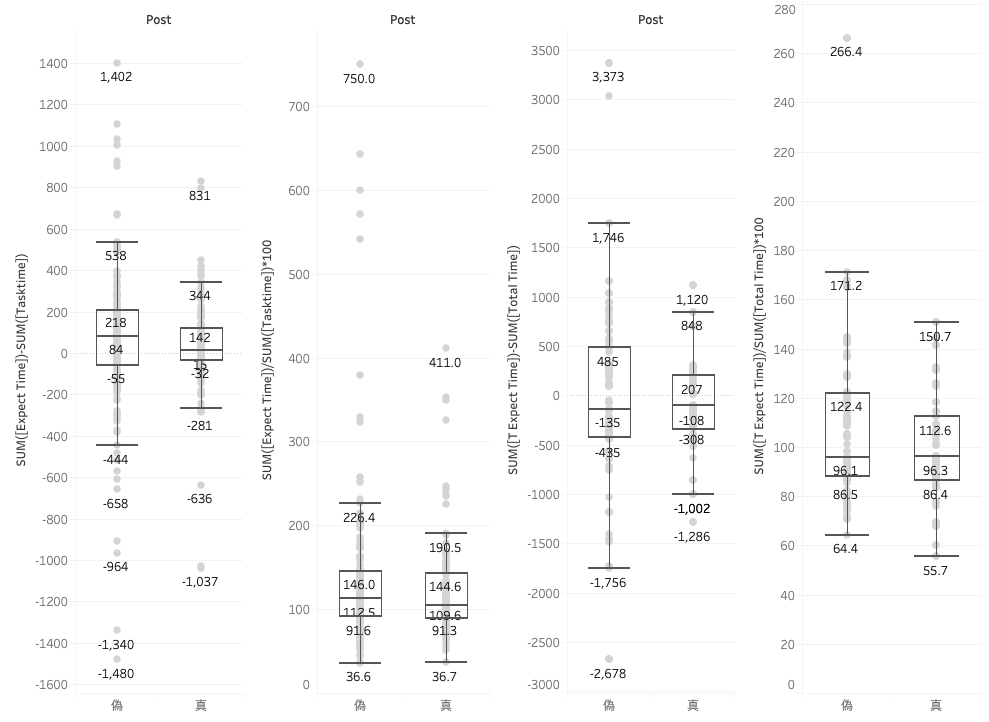
\includegraphics[width=15cm]{images/7/10.png}}
		\caption{ADLogger導入前後の比較(箱髭図)}
		\label{fig:10}
	\end{center}
\end{figure}


\begin{table}[ht]
\begin{center}
 \caption{平均と標準偏差によるADLogger導入前後比較}
\begin{tabular}{|c|c|c|c|c|} \hline
 & タスク時間(秒) & タスク時間(\%) & 総合時間(秒) & 総合時間(\%) \\ \hline 
平均(導入前)& 28.12& 136.59 & -21.37& 105.89 \\ \hline
平均(導入後)& 20.46& 121.24 & -49.89& 100.98 \\ \hline
標準偏差(導入前)& 193.02& 102.47 & 460.50& 29.10 \\ \hline
標準偏差(導入後)& 169.93& 62.55 & 356.20& 25.37 \\ \hline
\end{tabular}
  \label{tb:ave}
\end{center}
\end{table}

\begin{figure}[ht]
	\begin{center}
	\fbox{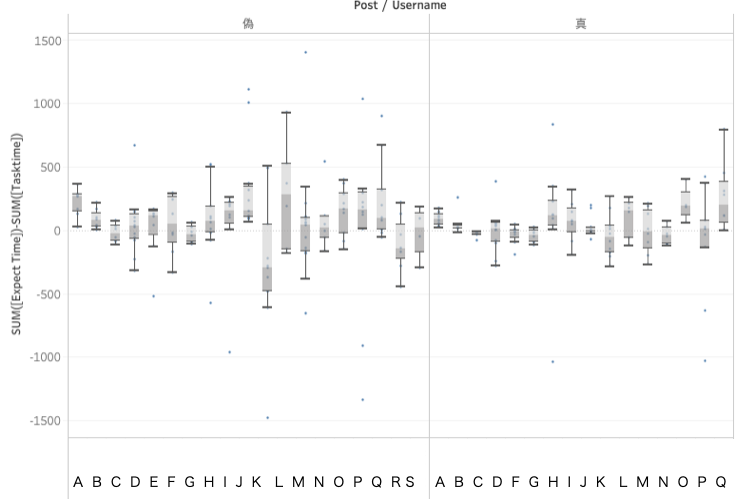
\includegraphics[width=15cm]{images/7/11.png}}
		\caption{ADLogger導入前後の比較(タスク時間(秒))}
		\label{fig:11}
	\end{center}
\end{figure}

\begin{figure}[ht]
	\begin{center}
	\fbox{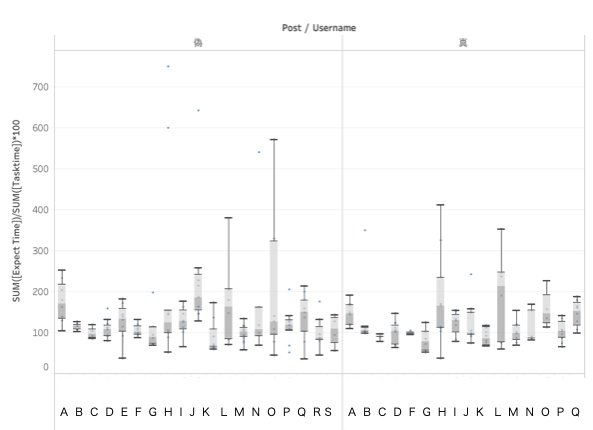
\includegraphics[width=15cm]{images/7/12.png}}
		\caption{ADLogger導入前後の比較(タスク時間(\%))}
		\label{fig:12}
	\end{center}
\end{figure}

\begin{figure}[ht]
	\begin{center}
	\fbox{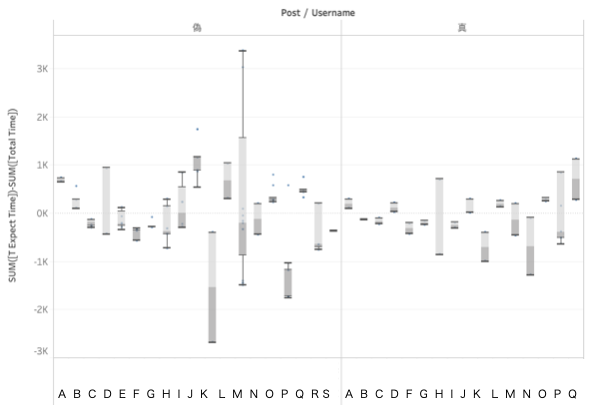
\includegraphics[width=15cm]{images/7/13.png}}
		\caption{ADLogger導入前後の比較(総合時間(秒))}
		\label{fig:13}
	\end{center}
\end{figure}

\begin{figure}[ht]
	\begin{center}
	\fbox{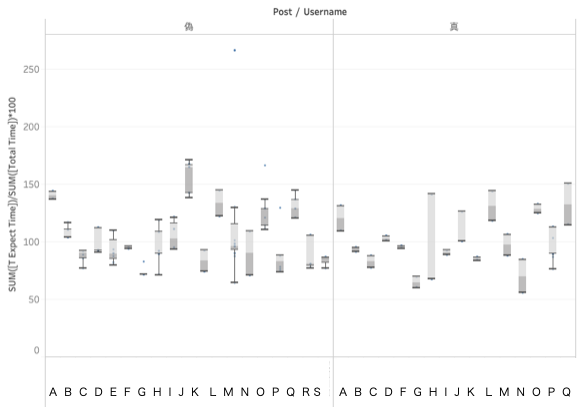
\includegraphics[width=15cm]{images/7/14.png}}
		\caption{ADLogger導入前後の比較(総合時間(\%))}
		\label{fig:14}
	\end{center}
\end{figure}




\subsection{インタビューについて}
本項では見積もり傾向から図~\ref{fig:compare}の見積もりの係数が高い順の
上位6人をグループ\UTF{2460},中位上位6人をグループ\UTF{2461},下位7人をグループ\UTF{2462}とした上で
被験者を下記の様に分け,インタビューの質問項目など違いを調査した.

結果,特筆されるのはまず苦手意識に関してはグループ\UTF{2460}の方が苦手意識を感じている被験者が相対的に少なく,\UTF{2461}・\UTF{2462}の被験者に苦手意識を感じている被験者が多かった.
また,見積もりを意図的に長く申告し少しゆとりを持たせている被験者はグループ\UTF{2460}・\UTF{2462}の被験者が多く,逆に\UTF{2461}に時間にゆとりを持たせて申告している被験者はいなかった.
また,13人の被験者からはタイマー・予測時間の可視化によって安心感の向上や時間に対する効率化の意識の向上が発生したと述べていた.

尚,インタビューの詳細を以下に記す.
問1に関しては「長い」と答えた人の中には「余裕を持ちたい為」と回答していた.
「定刻通り」と答えた人は「なんとなく」「勘」と言った感覚知による見積もりを主旨する意見が上がった.
「短い」と答えた人は「長く見積もるとその分伸びてしまう為」と言った声が上がった.
問3で「はい」と答えた人は「オフの日は家族と会話する」「お風呂に入るタイミングが被ってしまい家族が出るまで別のことを行った」と回答した人がいた.
問5で連続していないルーティンの人は別の作業を主目的に行うことが多く,例として「間にオンラインミーティングが入る場合がある」「コードを書く」「課題に向けた作業を行う」などが挙げられた.
問6では行うタスク,タスクの時間,タスク間の時間で変わる人が見受けられた.
問7に関しては「zoomで実験者を待たせてはいけない気持ちになった」「いつもは行うタスクがバラバラだが実験のためにタスクを固定した」「タスク間の隙間を縮めてまとめた」と言った声があった.
問8に関して効果があったと答えた人は「時間が可視化され安心感が得られた」「時間が可視化され自分の行動が分かったことがためになった」
「テキパキと動きたいという動機付けにつながった」「タイマーの時計をよく見て時間を意識した」と言った意見があった.
効果がなかったと答えた人は「そもそもあまり閲覧しなかった」「UI面の手間が大きかった」「行動が慣れているため」などが挙げられた.
問9は「アプリの操作」や「実験を重ねるうちに」慣れが生じて実験に影響がでた可能性があると話していた.
問10は固定バッファ時間を設定した人はおらず,一部の人が変動バッファモードの値を初期値の「ゆっくり」から「やや急ぎ」「ややゆっくり」に変えていた.
問11に関して「信憑性が薄い」と答えた人は「ストップウォッチの存在で予測値に実測値を近づけたい心理が生まれるのであくまで理想値に過ぎないのでは」と回答した.
問12においてシステムのメリットは「機能がシンプルで分かりやすい点」「普段意識していなかった時間を意識しテキパキ動く効果がある点」
「ストップウォッチで時間の経過が見られる点」などが主に挙げられた.
デメリットは「生活が不規則・ルーティンが定まっていない為自分の生活とアプリの行動変容目的が合わない」「UI面・デザイン」を主に述べており,
UIに関して問13では「AppleWatchであれば」「音声操作が良い」「時間を登録することへの手間の軽減」「オン/オフ以外のグラデーションが必要」「リマインダーとの連携」
「計測登録後タイマー画面に自動で戻る」「ずっと起動しなくても裏で計測できるようにする」
と言った意見が解決案として寄せられた.
問13の他の意見としては「朝の支度ではなく勉強用に使いたい」「引越しなど環境に変化があれば」「平日なら」と言った声が上がった.

\section{考察}
\subsection{アプリケーションの効果について}
実験結果から,ADLogger機能導入によって見積もりの予測時間と実測時間の差が縮まる効果が得られた.特に時間管理に対し苦手意識のある被験者や見積もりの係数が1に近い被験者程効果が大きかった.
一方,ADLogger導入後に見積もりの時間を変更した人はわずか3人である点,インタビューにて時間を意識すると述べている被験者が多かった事から本アプリケーションは
「見積もり傾向から自分の精度の悪い見積もりを修正する事によってズレが少なくなる」のではなく,「時間傾向の可視化に対しタイマーのカウントアップによって時間をより合わせる」効果をより発揮していると考えられる.

また,傾向線で見ると下振れしている被験者が多い事から,本機能の用いたバッファの取り方では見積もりを少なく見積もる様になってしまう可能性があり,バッファや目標時間は本機能の提示では正しく導けない事が分かる.
これは被験者別に傾向のタイプ分けをせず,かつまだ前例の無い中での暫定的な見積もりの提示をしており,より最適化が求められると考えられる.

\subsection{タイプ分けについて}
見積もり係数で分けた3グループ毎にADLoggerの効果に差がある事から,朝の準備に対し時間を見積もり,行動するパターンも少なくとも3パターンはあると考えられる.ここでは見積り係数の3グループを元に傾向を述べる.

グループ\UTF{2460}の被験者は見積りの時間を意識的に長く見積もる傾向にあり,見積り方はタスク自体を多めに見積もる人とバッファとして追加で数分余裕を持たせる人がいる.
グループ\UTF{2460}は時間が余ることは既に想定内であり実際に時間が余った時のみ追加でやる事なども合わせて考えた上で行動を行い,ゆとりがある事を前提として行動を見積もる.時間管理に対して苦手意識は感じない人が多い.
グループ\UTF{2461}の被験者は見積りの時間を実測値と丁度同じくらいに見積もる傾向にあり,本人の見積り方にバッファが存在しない事が多く,時間管理に対し苦手意識を感じる被験者が特に多い.
グループ\UTF{2462}の被験者は大抵は実測値の方が見積もりより長くかかる傾向にあるが,時間管理に対して苦手意識は感じない人と感じる人がいる.

実験によって大きく効果が出たのは\UTF{2461}\UTF{2462}である.
特にグループ\UTF{2461}においては大多数が見積もり時間ぴったりに見積もり,バッファの概念が無くかつ苦手意識がある事から
グループ\UTF{2461}に本システムを導入する事によって遅刻のリスクを十分に減らす可能性がある.
また,グループ\UTF{2460}\UTF{2462}においても「普段無意識に行っている時間の可視化」及び「システム導入による効率化向上の動機付け」によってシステムに効果を感じたユーザも大きかった.
グループ\UTF{2460}\UTF{2461}\UTF{2462}それぞれ異なった効果でありつつも一定の効果を得られた.